\documentclass[a4paper,12pt]{book}
\usepackage[utf8]{inputenc}
\usepackage{graphicx}

\begin{document}

\author{Radu Ciobanu}


\title{Formalization of regular languages and their properties}
\date{May 2014}

\frontmatter
\maketitle
\chapter*{Abstract}
This research project is based on formally proving mathematical properties of regular languages from the theory of automata. Our development has been done in the dependently-typed Coq proof assistant. Our constructive proofs include notions of languages, finite automata (including \textit{conversions} between deterministic and nondeterministic),  the \textit{equivalence} between finite automata and regular expressions, and also some useful theorems that help us see whether a language is regular, i.e the pumping lemma and the Myhill-Nerode theorem. Also, we have formalised the concept of \textit{automata minimization}.

In order to deal with finite types, we have implemented our own library that formalises some of the main mathematical results that refer to finiteness. 
\tableofcontents
\chapter{ Introduction}
In the literature, automata theory first appeared as an interdisciplinary field, comprising notions from mathematics, computer science and electrical engineering. 

This field is developed on the model of “abstract machines” called automatas, that are able to compute values given an input represented by words. Also, different variants of them (Turing Machines) are extensively used in the decision whether a problem can be solved in reasonable amount of time (NP-completeness problems).

The main goal of the project is to develop a mathematical formalization of properties from regular languages by using the Coq dependently-typed proof assistant. These notions are highly relevant to pure mathematics, artificial intelligence, linguistics, etc.
\chapter{Type theory}
The concept of type theory is vital in the understanding of mathematical logic and theoretical computer science. It focuses on the question of “what exactly is a proof”. The importance of a type is based on clarity and absence of wrong definitions. A formalism is a pure, rigorous presentation in which we need to manipulate symbols and their meaning.

 We can observe a resemblance between a formalism and principles from Plato's philosophy. Both describe pure, ideal thinking and the existence of the objects described will not lead to contradictions. Classical logic, developed in the Greek antiquity comprises the law of excluded middle.It is represented as p \verb+\+/ not p , where p is a proposition. This means that a statement can be either true or false. As an example, one can state simple facts like “It is raining or it’s not raining”- and be a true proposition.
Dutch mathematician L.E.Jan Brouwer founded intuitionism, a concept that didn’t use the notion of excluded middle. The main idea is that in order to provide a proof we have to explicitly construct a proof object, e.g for a binary conjuction A /\verb+\+ B we must construct a pair of proof objects , one object for each construct.

Each logical system requires connectives(like conjuncti-on, disjunction, quantifiers, etc..). For intuitionism, the meaning of connectives will be used taking into account one of the most fundamental mathematical concept- construction. A certain fact X will be established using construction. For instance, in basic arithmetic, in order to prove that 1+2 = 3, we will do the following: we construct 1, we construct 2, then we compare the outcome with the result of the construction of 3. The outcome will be a confirmation of the equation from above. The notation “p : P ” will tell us that “p is the construction that establishes P” or, other put, “p is a proof of P”. As we stated above, a proof of A /\verb+\+ B is made of 2 proofs a:A and b:B.

Negation is defined as p: $not$ A. It will tell us that each proof a: A will be transformed by the proof p into a contradiction(i.e A $\to $ False).

A proof of $not$ A says that A has no proof. As a remark, Brouwer developed an intuitionistic proof of $not$($not$($not$A)) $<=>$ $not$ A.

In order to prove disjunction, we construct a pair (a1 , a2) –where a1 will keep the information of which disjunct is correct and a2 will be the proof of either A or B. In fig.1, we observe that if B is false, then a1 =0. Therefore a2 will be the proof of A. The same reasoning applies if A is false.

In the intuitionistic approach, the implication propositional connective (A $\to$ B) is based on the notion of proof, requiring a definition of proof a : (A $\to$ B), taking into account the proofs of A and B. A $to$ B will be correct if we can prove B as soon as the correctness of A has been realised. Using proofs, p: A $\to $ B if p transforms each proof of q: A into a proof p (q ) : B.

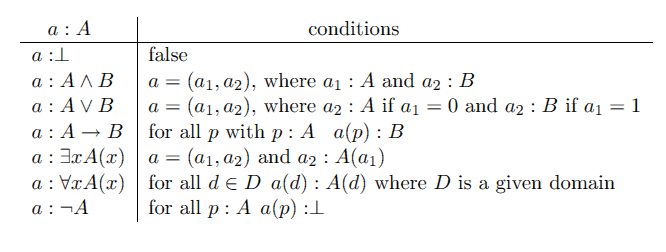
\includegraphics[scale=0.6]{graph/intlog}

\subsection{Natural deduction}
Gerhard Gentzen introduced a new kind of formalization of logic, based on previous work in the field, a majority of it being presented above. It is called “natural deduction”. The Coq programming language uses it in the development of its tactics. A programmer can prove certain facts by using specific tactics that are associated with logic rules.

\paragraph{Rules}


This formula is called conjunction-introduction. It says that if we know A and we know B, then we can conclude that A /\verb+\+ B is true.

It is called conjunction elimination. It says that if we know that A /\verb+\+ B is true then we may state that both A and B are true.
\backmatter
% bibliography, glossary and index would go here.

\end{document}